\chapter{}
\section{Diffuse and Specular Scene Renderings}
\label{sec:diffuse_and_specular_scene_renderings}
Figure \ref{fig:diffuse_specular_breakdown} shows the breakdown of the reference and \ac{lod} image into the diffuse and specular component as referenced in Section \ref{chap:results_and_discussion}.
\begin{figure}[ht]
    \centering
    \begin{subfigure}[b]{0.49\linewidth}
        \centering
        \includegraphics[width=1\linewidth]{img/results/diffuse_only_mesh.jpg}
        \caption{}
        % \label{fig:render_comparison_mesh}
    \end{subfigure}
    \begin{subfigure}[b]{0.49\linewidth}
        \centering
        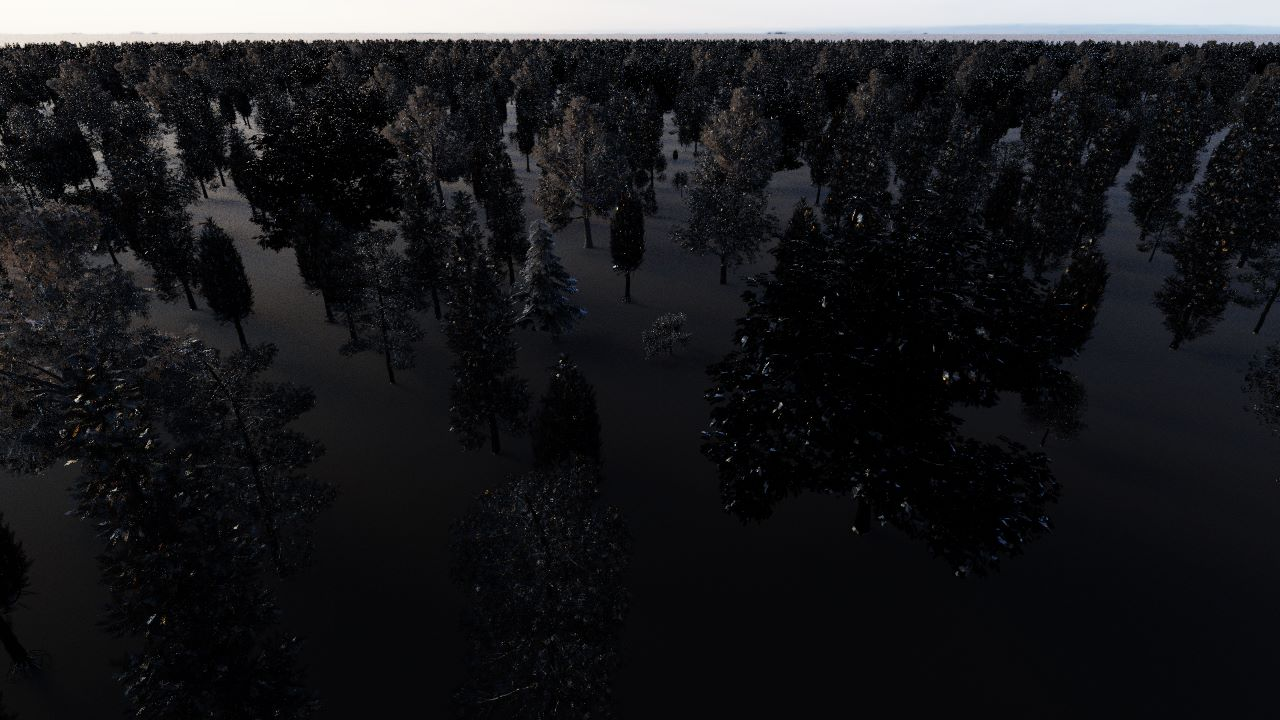
\includegraphics[width=1\linewidth]{img/results/specular_only_mesh.jpg}
        \caption{}
        % \label{fig:render_comparison_lod}
    \end{subfigure}
    \begin{subfigure}[b]{0.49\linewidth}
        \centering
        \includegraphics[width=1\linewidth]{img/results/diffuse_only_lod_1A.jpg}
        \caption{}
        % \label{fig:render_comparison_mesh}
    \end{subfigure}
    \begin{subfigure}[b]{0.49\linewidth}
        \centering
        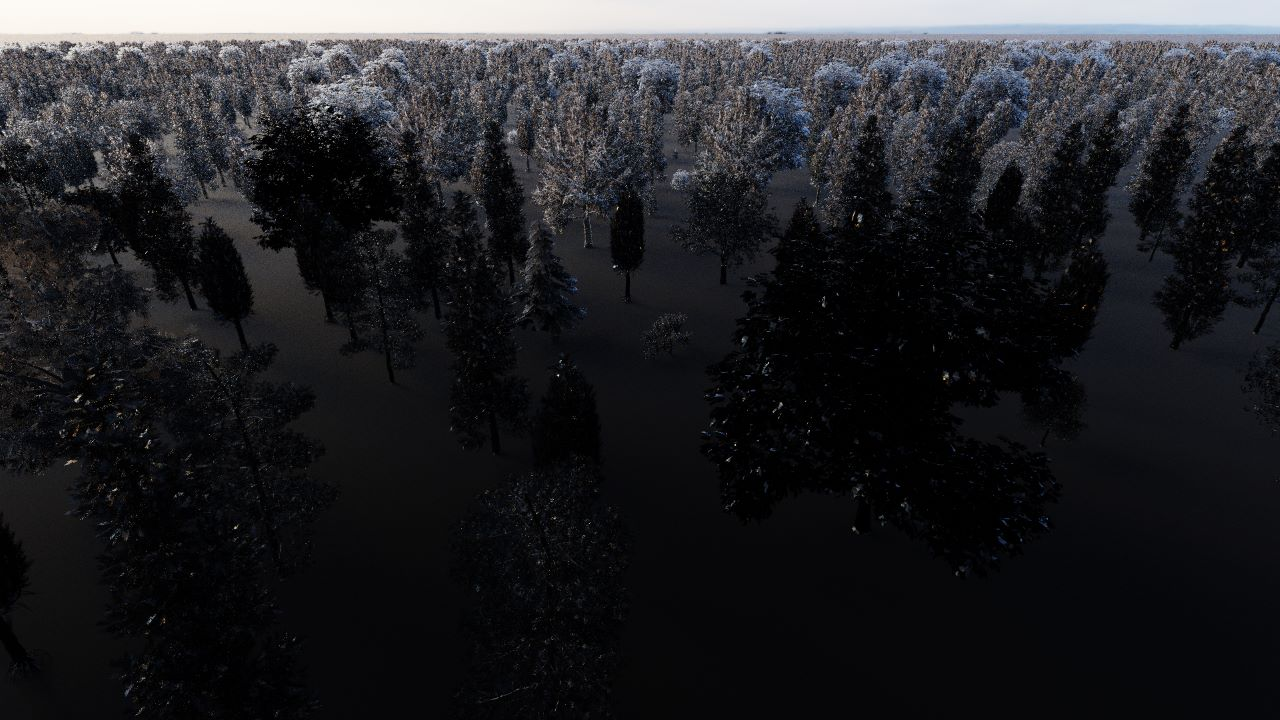
\includegraphics[width=1\linewidth]{img/results/specular_only_lod_1A.jpg}
        \caption{}
        % \label{fig:render_comparison_lod}
    \end{subfigure}
    % \caption[Comparison between mesh and volume renderings of the forest]{Renderings of the forest using meshes only (a) and using \acsp{lod} if a voxel is smaller than a pixel (b).}
    \caption[Diffuse and specular components rendered seperately]{(a) and (b) show the diffuse respectively specular component of the reference image, (c) and (d) show the diffuse respectively specular component when using \acsp{lod} where a voxel covers at most one pixel.}
	\label{fig:diffuse_specular_breakdown}
\end{figure}

\section{\acs{psnr} and \acs{ssim} Image Errors}
\label{sec:psnr_and_ssim_errors}
In the following we provide the \ac{psnr} and \ac{ssim} errors for the different combinations between the number of covered pixels and the minimum \ac{lod} size.

The \ac{psnr} values (in dB) are:
\begin{center}
    \begin{tabular}{| c | c | c | c | c | c | c | c | c |}
        \cline{3-9}
        \multicolumn{2}{c|}{} & \multicolumn{7}{c|}{Minimum voxel size [m]} \\
        \cline{3-9}
        \multicolumn{2}{c|}{} & 0.1 & 0.2 & 0.4 & 0.8 & 1.6 & 3.2 & 6.4 \\
        \hline
        \multirow{4}{*}{Covered pixels}& 1 & 21.9 & 22.8 & 23.5 & 23.8 & 23.9 & 23.9 & 23.9 \\
        \cline{2-9}
        & 4 & 21.2 & 21.9 & 22.7 & 23.4 & 23.7 & 23.9 & 23.9 \\
        \cline{2-9}
        & 9 & 19.8 & 21.2 & 22.1 & 22.9 & 23.5 & 23.8 & 23.9 \\
        \cline{2-9}
        & 16 & 19.6 & 20.9 & 21.6 & 22.5 & 23.3 & 23.7 & 23.9 \\
        \hline
    \end{tabular}
\end{center}

The \ac{ssim} values are:
\begin{center}
    \begin{tabular}{| c | c | c | c | c | c | c | c | c |}
        \cline{3-9}
        \multicolumn{2}{c|}{} & \multicolumn{7}{c|}{Minimum voxel size [m]} \\
        \cline{3-9}
        \multicolumn{2}{c|}{} & 0.1 & 0.2 & 0.4 & 0.8 & 1.6 & 3.2 & 6.4 \\
        \hline
        \multirow{4}{*}{Covered pixels}& 1 & 0.573 & 0.632 & 0.665 & 0.679 & 0.685 & 0.685 & 0.685 \\
        \cline{2-9}
        & 4 & 0.502 & 0.563 & 0.626 & 0.663 & 0.678 & 0.684 & 0.685 \\
        \cline{2-9}
        & 9 & 0.396 & 0.501 & 0.586 & 0.639 & 0.668 & 0.680 & 0.685 \\
        \cline{2-9}
        & 16 & 0.367 & 0.475 & 0.545 & 0.616 & 0.658 & 0.675 & 0.683 \\
        \hline
    \end{tabular}
\end{center}